\documentclass[a4paper,12pt]{article}
\usepackage{a4wide,tikz}
\usepackage[landscape]{geometry}
\parindent=0cm
\begin{document}
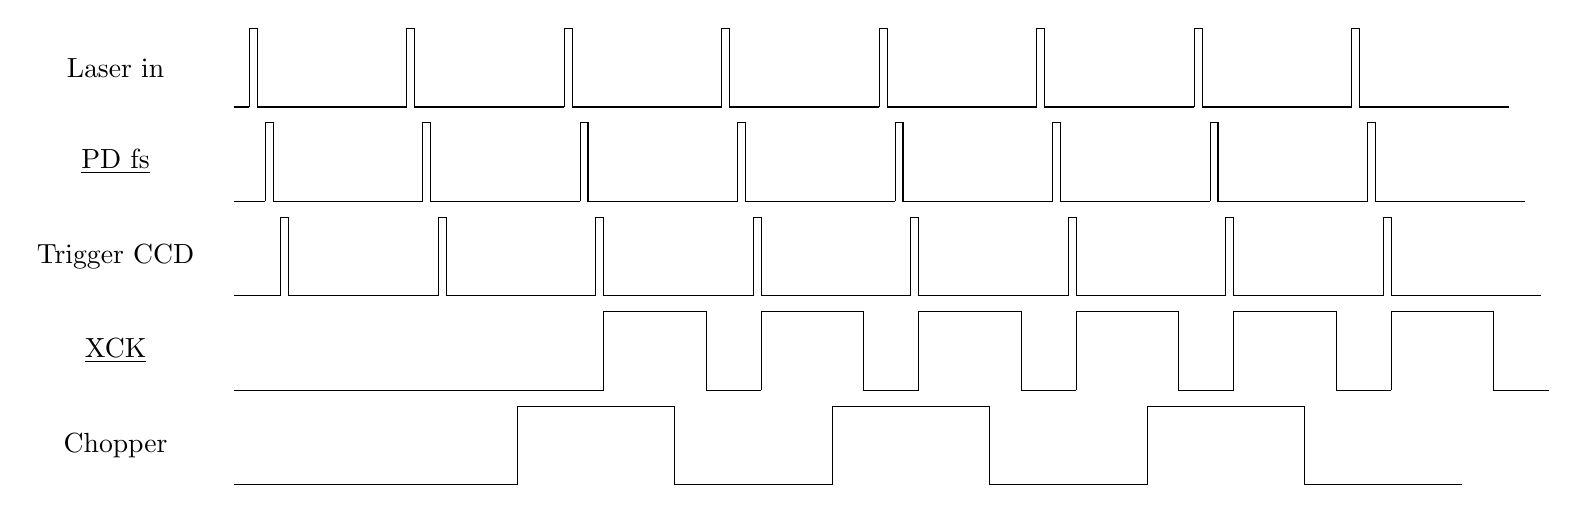
\begin{tikzpicture}
  \def\yin{4.8}
  \def\yfs{3.6}
  \def\yccd{2.4}
  \def\yxck{1.2}
  \def\ychop{0}
  \draw (0,\yin) -- ++(0.2,0);
  \foreach \x in {0.2,2.2,...,14.2}
    \draw (\x,\yin) -- ++(0,1) -- ++(0.1,0) -- ++(0,-1) -- ++(1.9,0);
%  \draw (16,\yin) -- ++(1.9,0);
  \draw(-1.5,\yin+0.5) node {Laser in};
  %
  \draw (0,\yfs) -- ++(0.4,0);
  \foreach \x in {0.4,2.4,...,14.4}
    \draw (\x,\yfs) -- ++(0,1) -- ++(0.1,0) -- ++(0,-1) -- ++(1.9,0);
%  \draw (16.2,\yfs) -- ++(1.7,0);
  \draw(-1.5,\yfs+0.5) node {\underline{PD fs}};
  %
  \draw (0,\yccd) -- ++(0.6,0);
  \foreach \x in {0.6,2.6,...,14.6}
    \draw (\x,\yccd) -- ++(0,1) -- ++(0.1,0) -- ++(0,-1) -- ++(1.9,0);
%  \draw (16.4,\yccd) -- ++(1.5,0);
  \draw(-1.5,\yccd+0.5) node {Trigger CCD};
  %
  \draw (0,\yxck) -- ++(4.7,0);
  \foreach \x in {4.7,6.7,...,14.7}
    \draw (\x,\yxck) -- ++(0,1) -- ++(1.3,0) -- ++(0,-1) -- ++(0.7,0);
%  \draw (17.8,\yxck) -- ++(0.1,0);
  \draw(-1.5,\yxck+0.5) node {\underline{XCK}};
  %
  \draw (0,\ychop) -- ++(3.6,0);
  \foreach \x in {3.6,7.6,11.6}
    \draw (\x,\ychop) -- ++(0,1) -- ++(2,0) -- ++(0,-1) -- ++(2,0);
%  \draw (16.9,\ychop) -- ++(1,0);
  \draw(-1.5,\ychop+0.5) node {Chopper};
  %
\end{tikzpicture}
\smallskip

a)\\
\begin{tikzpicture}
  \def\ytrigps{1.2}
  \def\yps{0}
  \draw (0,\ytrigps) -- ++(3.8,0);
  \foreach \x in {3.8,7.8,11.8}
    \draw (\x,\ytrigps)-- ++(0,1) -- ++(0.3,0) -- ++(0,-1) -- ++(3.7,0);
%  \draw (16.4,\ytrigps) -- ++(1.9,0);
  \draw(-1.5,\ytrigps+0.5) node {\underline{Trigger ps}};
  %
  \draw (0,\yps) -- ++(4.1,0);
  \foreach \x in {4.1,8.1,12.1}
    \draw (\x,\yps) -- ++(0,1) -- ++(0.1,0) -- ++(0,-1) -- ++(3.9,0);
%  \draw (16.4,\yps) -- ++(1.9,0);
  \draw(-1.5,\yps+0.5) node {\underline{PD ps}};
  %
\end{tikzpicture}
\smallskip

b)\\
\begin{tikzpicture}
  \def\ytrigps{1.2}
  \def\yps{0}
  \draw (0,\ytrigps) -- ++(3.8,0);
  \foreach \x in {3.8,7.8,11.8}
    \draw (\x,\ytrigps)-- ++(0,1) -- ++(0.3,0) -- ++(0,-1) -- ++(3.7,0);
%  \draw (16.4,\ytrigps) -- ++(1.9,0);
  \draw(-1.5,\ytrigps+0.5) node {\underline{Trigger ps}};
  %
  \draw (0,\yps) -- ++(4.1,0);
  \foreach \x in {4.1,8.1,12.1}
    \draw (\x,\yps) -- ++(0,1) -- ++(0.1,0) -- ++(0,-1) -- ++(3.9,0);
%  \draw (16.4,\yps) -- ++(1.9,0);
  \draw(-1.5,\yps+0.5) node {\underline{PD ps}};
  %
\end{tikzpicture}
\end{document}
